\section{Lie Groups and Lie Algebras}

  \begin{definition}
    A \textbf{Lie group} is a group $\mathcal{G}$ that is also a finite-dimensional smooth manifold, in which the group operations of multiplication and inversion are smooth maps. Smoothness of the group multiplication
    \begin{equation}
      \mu: \mathcal{G} \times \mathcal{G} \rightarrow \mathcal{G}, \; \mu(x, y) = x y
    \end{equation}
    means that $\mu$ is a smooth mapping of the product manifold $\mathcal{G} \times \mathcal{G}$ into $\mathcal{G}$. These two requirements can be combined to the single requirement that tahe mapping 
    \begin{equation}
      (x, y) \mapsto x^{-1} y
    \end{equation}
    be a smooth mapping of the product manifold into $\mathcal{G}$. 
  \end{definition}

  \begin{definition}
    A \textbf{Lie Algebra} is a vector space $\mathfrak{g}$ with an operation called the \textbf{Lie Bracket} 
    \begin{equation}
      [\cdot, \cdot]: \mathfrak{g} \times \mathfrak{g} \rightarrow \mathfrak{g}
    \end{equation}
    Satisfying
    \begin{enumerate}
      \item Bilinearity: $[ax + by, z] = a[x,z] + b[y,z], \; [z, ax + by] = a[z, x] + b[z,y]$
      \item Anticommutativity: $[x,y] = -[y,x]$
      \item Jacobi Identity: $[x,[y,z]] + [y,[z,x]] + [z,[x,y]] = 0$
    \end{enumerate}
    Clearly, this implies that $\mathfrak{g}$ is a nonassociative algebra. Note that a Lie Algebra does not necessarily need to be an algebra in the sense that there needs to be multiplication operation that is closed in $\mathfrak{g}$. 
  \end{definition}

  \begin{example}
    A common example of a Lie Braket in the algebra of matrices is defined
    \begin{equation}
      [A, B] \equiv AB - BA
    \end{equation}
    called the \textbf{commutator}. Note that in this case, the definition of the Lie bracket is dependent on the definition of the matrix multiplication. Without defining the multiplication operation, we wouldn't know what $AB$ or $BA$ means. Therefore, we see that the Lie algebra of $n \times n$ matrices has three operations: matrix addition, matrix multiplication, and the commutator (along with scalar multiplication). But in general, it is not necessary to have that multiplication operation for abstract Lie algebras. $\mathfrak{g}$ just needs to be a vector space with the bracket.  
  \end{example}

  \begin{example}
    The set of all symmetric matrices is a vector space, but it is \textbf{not} a Lie algebra since the commutator $[A,B]$ is not symmetric unless $A B = B A$. 
  \end{example}

  We will first talk about groups of matrices as a more concerete example before we get into abstract Lie groups. Recall that the matrix exponential map is defined
  \begin{equation}
    exp: \text{Mat}(n, \mathbb{C}) \rightarrow \text{mat}(n, \mathbb{C}), \; exp(A) = e^A = \sum_{p \geq 0} \frac{A^p}{p!}
  \end{equation}
  Note that this value is always well defined. This lets us define
  \begin{equation}
    exp(t A) \equiv e^{t A} \equiv I + tA + \frac{1}{2} t^2 A^2 + \frac{1}{3!} t^3 A^3 + ... 
  \end{equation}
  where if $t$ is small, we can expect a convergence. Note that exp maps addition to multiplication. That is, we can interpret it as a homomorphism from 
  \begin{equation}
    exp: \mathfrak{g} \rightarrow \mathcal{G}
  \end{equation}
  where $\mathfrak{g}$ is the Lie algebra and $\mathcal{G}$ is the Lie group (which we will treat just as a matrix group). To find the inverse of the exponential map, we can take the derivative of $e^{tA}$ at $t=0$. That is, 
  \begin{align*}
    \bigg(\frac{d}{d t} e^{tA} \bigg) \bigg|_{t=0} & = \bigg(\sum_{k=0}^\infty \frac{1}{k!} t^k A^{k+1} \bigg) \bigg|_{t=0} = A
  \end{align*}
  So, the mapping
  \begin{equation}
    \frac{d}{dt} \bigg|_{t=0}: \mathcal{G} \rightarrow \mathfrak{g}
  \end{equation}
  maps the Lie group back to the algebra. We can interpret this above mapping by visualizing the Lie Algebra as a tangent (vector) space of the abstract Lie group $\mathcal{G}$ at the identity element of the Lie group. The visualization below isn't the most abstract one, but it may help:

  \begin{figure}[H]
    \centering 
    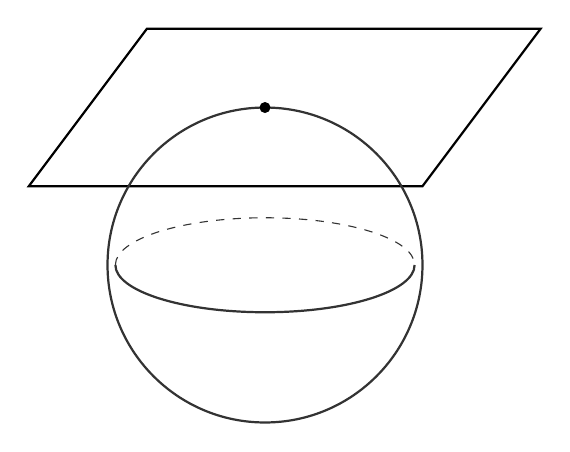
\begin{tikzpicture}[scale=1]
      % Define colors
      \colorlet{spherecol}{black!80}
      \colorlet{arrowcol}{cyan!70!blue}
      
      % Draw the tangent plane (Lie Algebra)
      \draw[thick] (-1.5,3) -- (3.5,3) -- (2,1) -- (-3,1) -- cycle;
      
      % Draw the sphere (Lie Group)
      \draw[spherecol, thick] (0,0) circle (2cm);
      \draw[spherecol, thick] (-1.9,0) arc (180:360:1.9cm and 0.6cm);
      \draw[spherecol, dashed] (-1.9,0) arc (180:0:1.9cm and 0.6cm);
      
      % Identity element
      \fill (0,2) circle (0.07cm);
    \end{tikzpicture}
    \caption{The Lie algebra can be visualized as the tangent space at the identity.} 
    \label{fig:lie_algebra_tangent_space}
  \end{figure}

  For example, say that the Lie group $\mathcal{G}$ is a unit circle in $\mathbb{C}$, then the Lie algebra of $\mathcal{G}$ is the tangent space at the identity $1$, which can be identified as the imaginary line in the complex plane $\{i t \; | \; t \in \mathbb{R}\}$, with 
  \begin{equation}
    i t \mapsto exp(it) \equiv e^{it} \equiv \cos{t} + i \sin{t}
  \end{equation}

  \begin{center}
    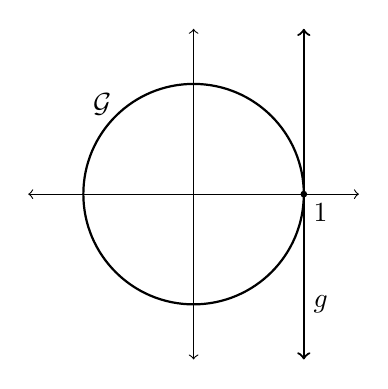
\begin{tikzpicture}[scale=0.7]
      \draw[thick] (0,0) circle (2);
      \node[below right] at (-2,2) {$\mathcal{G}$};
      \draw[<->] (-3,0)--(3,0);
      \draw[<->] (0,-3)--(0,3);
      \draw[fill] (2,0) circle (0.05);
      \node[below right] at (2,0) {$1$};
      \draw[thick, <->] (2,-3)--(2,3);
      \node[right] at (2,-2) {$\mathfrak{g}$};
    \end{tikzpicture}
  \end{center}
  So, analyzing the Lie group by looking at its Lie algebra turns a nonlinear problem to a linear one; this is called a \textbf{linearization} of the Lie group. The existence of this exponential map is one of the primary reasons that Lie algebras are useful for studying Lie groups. 

  \begin{example}
    The exponential map 
    \begin{equation}
      exp: \mathbb{R} \rightarrow \mathbb{R}^+, \; x \mapsto e^x
    \end{equation}
    is a group homomorphism that maps $(\mathbb{R}, +)$ to $(\mathbb{R}^+, \times)$. This means that $\mathbb{R}$ is the Lie algebra of the Lie group $\mathbb{R}^+$. 
  \end{example}

  \begin{theorem}
    If $A$ and $B$ are commuting square matrices, then 
    \begin{equation}
      e^{A + B} = e^A \, e^B
    \end{equation}
    In general, the solution $C$ to the equation
    \begin{equation}
      e^{A} \, e^B = e^C
    \end{equation}
    is given by the \textbf{Baker-Campbell-Hausdorff formula}, defined
    \begin{equation}
      C = A + B + \frac{1}{2}[A,B] + \frac{1}{12} [A,[A,B]] - \frac{1}{12} [B,[A,B]] + ...
    \end{equation}
    consisting of terms involving higher commutators of $A$ and $B$. The full series is much too complicated to write, so we ask the reader to be satisfied with what is shown. 
  \end{theorem}

  The BCH formula is messy, but it allows us to compute products in the Lie Group as long as we known the commutators in the Lie Algebra. 

  Therefore, we can describe the process of constructing a Lie group from a Lie Algebra (which a vector space) as such. We take a vector space $V$ and endow it the additional bracket operation. We denote this as
  \begin{equation}
    \mathfrak{g} \equiv (V, [\cdot, \cdot])
  \end{equation}
  Then, we take every element of $\mathfrak{g}$ and apply the exponential map to them to get an another set $\mathcal{G}$. We then endow a group structure on $\mathcal{G}$ by defining the multiplication as 
  \begin{equation}
    \cdot: \mathcal{G} \times \mathcal{G} \rightarrow \mathcal{G}, \; e^A \cdot e^B = e^{A * B}
  \end{equation}
  where $A*B$ is defined by the BCH formula up to a certain $k$th order. Since the $*$ operation is completely defined by the bracket in the Lie algebra, it tells us how to multiply in the Lie group. This process can be made more abstractly, depending on what $A, B$ and $[\cdot,\cdot]$ is, beyond matrices. 

\subsection{Lie Algebras of Classical Lie Groups}

  \begin{definition}[General Linear Group]
    The \textbf{general linear group}, denoted GL$(V)$, is the set of all bijective linear mappings from $V$ to itself. Similarly, GL$_{n}(\mathbb{F})$, or GL $(n, \mathbb{F})$ is the set of all nonsingular $n \times n$ matrices over the field $\mathbb{F}$. Due to the same dimensionality of the following spaces, it is clear that GL$(V) \simeq$ GL$(\mathbb{F}^{n}) \simeq$ GL$_{n}(\mathbb{F})$. The \textbf{special linear group}, denoted SL$_{n} (\mathbb{F})$ or SL$(n, \mathbb{F})$, is the set of $n\times n$ matrices a with determinant $1$. SL$_{n}(\mathbb{F})$ is a subgroup of GL$_{n}(\mathbb{F})$, which is a subset of the ring of all $n \times n$ matrices over field $\mathbb{F}$, denoted $\mathbb{L}_{n}(\mathbb{F})$. 
  \end{definition}

  \begin{definition}[Translation Group]
    The group of all translations in the space $V$ is denoted Tran$\,V$. Its elements are usually denoted as $t_{u}$, where $u$ is the vector that is being translated by. It can also be interpreted as shifting the origin by $-u$. It is clear that Tran$\,V \simeq V$. 
  \end{definition}

  \begin{definition}[General Affine Group]
    The \textbf{general affine group} is the pair of all transformations
    \begin{equation}
      \text{GA} (V) \equiv \text{Tran}(V) \times \text{GL}(V)
    \end{equation}
  \end{definition}

  \begin{definition}[Isometries]
    The \textbf{Euclidean group} of \textbf{isometries} in the Euclidean space $\mathbb{E}^{n}$ (with the Euclidean norm), denoted Isom$\, \mathbb{E}^{n}$ or $\mathbb{E}(n)$, consists of all distance-preserving bijections from $\mathbb{E}^{n}$ to itself, called \textbf{motions} or \textbf{rigid transformations}. It consists of all combinations of rotations, reflections, and translations. The \textbf{special Euclidean group} of all isometries that preserve the \textbf{handedness} of figures is denoted $\mathbb{SE}(n)$, which is comprised of all combinations rotations and translations called \textbf{rigid motions} or \textbf{proper rigid transformations}.
  \end{definition}

  \begin{definition}[Orthogonal Group]
    The \textbf{orthogonal group}, denoted $\O(n)$, consists of all isometries that preserve the origin, i.e. consists of rotations and reflections. The \textbf{special orthogonal group}, denoted SO$(n)$, is a subgroup of O$(n)$ consisting of only rotations. We can see that 
    \begin{equation}
      \text{O}(n)=\frac{\text{Isom}\, \mathbb{E}^{n}}{\text{Tran}\,V}
    \end{equation}
  \end{definition}

  \begin{definition}[Transitive]
    A transformation group $G$ is called \textbf{transitive} if for any $x, y \in X$, there exists a $\phi \in G$ such that $y = \phi(x)$. 
  \end{definition}

  \begin{example}
    Tran$(V)$ and GA$(V)$ are transitive groups. 
  \end{example}

  \begin{definition}[Congruence Classes]
    Let $X$ be a set and $G$ its transformation group on $X$. The way we define $G$ determines the \textbf{geometry} of $X$. More specifically, a figure $F_{1} \subset X$ is \textbf{equivalent} or \textbf{congruent} to $F_{2} \subset X$ iff there exists $\phi \in G$ such that $F_{2} = \phi (F_{1})$ (or equivalently, $F_{1} = \phi (F_{2})$). This is an equivalence relation since
    \begin{enumerate}
      \item $F \sim F$. 
      \item $F \sim H \implies H \sim F$. 
      \item $F \sim H, H \sim K \implies F \sim K$
    \end{enumerate}
    Two figures that are in the same equivalence class are known to be \textbf{congruent} with respect to the geometry of $X$ induced by $G$. 
  \end{definition}

  Clearly, if two figures are congruent in Euclidean geometry, then they are congruent in Affine geometry, since E$(n) \subset$ GA$(n)$. 


\subsubsection[Lie Algebras of SL(2, R) and SL(2, C)]{Lie Algebras of $\SL(2, \mathbb{R})$ and $\SL(2, \mathbb{C})$}

  Given the group $\SL(2, \mathbb{R})$, there must be a corresponding Lie algebra of matrices such that $g = e^A \in \SL(2, \mathbb{R})$. We attempt to find this Lie algebra. Let $g \in \SL(2, \mathbb{R})$, with $g = e^A$. So, if $\det{g} = 1$, what is the corresponding restriction on $A$ in the algebra? We use the following theorem. 

  \begin{theorem}
    \begin{equation}
      \det{(e^A)} = e^{\Tr{(A)}}
    \end{equation}
  \end{theorem}
  \begin{proof}
    Put $A$ in Jordan Normal Form: $A = S^{-1} J S \implies A^n = S^{-1} J^n S \implies exp(A) = S^{-1} exp(A) S \implies \det{(exp(A))} = \det{e^J}$. But since $J$ is upper trianglar, $J^n$ is upper triangular $\implies e^J$ is upper triangular, which implies that 
    \begin{equation}
      \det{e^J} = \prod_i e^{\lambda_i} = e^{\Tr{(J)}} = e^{\Tr{(A)}}
    \end{equation}
    since trace is invariant under a change of basis. 
  \end{proof}

  So, $\det{(e^A)} = 1 \implies \Tr{(A)} = 2 \pi i n$ for $n \in \mathbb{Z}$. Since we want to component connected to the identity, we choose $n=0$ meaning that $\Tr{(A)} = 0$. And we are done. That is, the Lie algebra of $\SL(2, \mathbb{R})$ consists of traceless $2 \times 2$ matrices, denoted $\mathfrak{sl}_2 \mathbb{R}$. $\mathfrak{sl}_2 \mathbb{R}$ has basis (chosen arbitrarily) 
  \begin{equation}
    \bigg\{ H = \begin{pmatrix}
    1&0\\0&-1
    \end{pmatrix}, X = \begin{pmatrix}
    0&1\\0&0
    \end{pmatrix}, Y = \begin{pmatrix}
    0&0\\1&0
    \end{pmatrix}\bigg\}
  \end{equation}
  and the identity in the Lie algebra is the zero matrix, which translates to the $2 \times 2$ identity matrix in the Lie group. 
  \begin{equation}
    exp \begin{pmatrix}
    0&0\\0&0
    \end{pmatrix} = I
  \end{equation}
  We must not forget to define the bracket structure in $\mathfrak{sl}_2 \mathbb{R}$, so we define it as the commutator, which gives the identity
  \begin{align*}
    & [H,X] = HX - XH = 2X \\
    & [H,Y] = HY - YH = -2Y \\
    & [X,Y] = XY - YX = H
  \end{align*}
  Note that regular matrix multiplication is not closed within this Lie algebra. For example, 
  \begin{equation}
    X Y = \begin{pmatrix}
    1&0\\0&0
    \end{pmatrix}
  \end{equation}
  is clearly not traceless. However, the bracket operation keeps the matrices within this traceless condition (and thus, within this algebra), so you can't just stupidly multiply matrices together in a Lie algebra. Remember that regular matrix multiplication does not have anything to do with the Lie bracket and does not apply to this group. This algebra also simplifies the multiplicative inverse of a group to a simple additive inverse, making calculations easier. 

  Similarly, the Lie algebra of $\SL(2, \mathbb{C})$ also has the same basis 
  \begin{equation}
    \bigg\{ H = \begin{pmatrix}
    1&0\\0&-1
    \end{pmatrix}, X = \begin{pmatrix}
    0&1\\0&0
    \end{pmatrix}, Y = \begin{pmatrix}
    0&0\\1&0
    \end{pmatrix}\bigg\}
  \end{equation}
  but we choose the field to be $\mathbb{C}$, meaning that we take complex linear combinations rather than real linear ones. 

\subsubsection[Lie Algebra of SU(2)]{Lie Algebra of \(\SU(2)\)}

  $g \in $ SU$(2) \implies \det{g} = 1 \implies \Tr{A} = 0$. We also see that by definition $e^A$, 
  \begin{equation}
    (e^A)^\dagger = e^{A^\dagger} \text{ and } (e^A)^{-1} = e^{-A}
  \end{equation}
  which implies that $A^\dagger = - A$. That is, the unitary condition implies that the Lie algebra elements in $\mathfrak{su}(2)$ are traceless, anti-self adjoint $2 \times 2$ matrices over $\mathbb{C}$. 

  \begin{definition}
    The \textbf{Pauli matrices} are the three matrices
    \begin{equation}
      \bigg\{ \sigma_x = \begin{pmatrix}
      0&1\\1&0
      \end{pmatrix}, \sigma_y = \begin{pmatrix}
      0&-i\\i&0
      \end{pmatrix}, \sigma_z = \begin{pmatrix}
      1&0\\0&-1
      \end{pmatrix}\bigg\}
    \end{equation}
    Note that with some calculation, 
    \begin{align*}
      & [\sigma_x, \sigma_y] = 2 i \sigma_z \\
      & [\sigma_y, \sigma_z] = 2 i \sigma_x \\
      & [\sigma_z, \sigma_x] = 2 i \sigma_y
    \end{align*}
  \end{definition}

  To identify the basis of $\mathfrak{su}(2)$, we take the Pauli matrices and let 
  \begin{align*}
    & A_x \equiv - \frac{i}{2} \sigma_x = \begin{pmatrix} 0&-i/2\\-i/2&0 \end{pmatrix} \\
    & A_y \equiv - \frac{i}{2} \sigma_y = \begin{pmatrix}0&-1/2\\1/2&0\end{pmatrix} \\
    & A_z \equiv -\frac{i}{2} \sigma_z = \begin{pmatrix}-i/2&0\\0&i/2\end{pmatrix}
  \end{align*} 
  be the basis of $\mathfrak{su}(2)$. Clearly, $A_x, A_y, A_z$ are all traceless, anti-self adjoint $2 \times 2$ matrices. Moreover, they also satisfy
  \begin{align*}
    & [A_x, A_y] = A_z \\
    & [A_y, A_z] = A_x \\
    & [A_z, A_x] = A_y
  \end{align*}
  However, note that the algebra $\mathfrak{su}(2)$ consists of all \textbf{real} linear combinations of $A_x, A_y, A_z$. That is, $\mathfrak{su}(2)$ is a 3 dimensional \textbf{real} vector space, even though it has basis elements containing complex numbers. 

  However, we can always complexify this space by simply replacing real scalar multiplication in $\mathfrak{su}(2)$ with complex scalar multiplication. By complexifying $\mathfrak{su}(2)$, the Lie group SU$(2)$ formed by taking the exponential map on this complexified space is actually identical to $\SL(2, \mathbb{C})$. Indeed, this is true because first, the basis $\{H, X, Y\}$ of $\mathfrak{sl}_2 \mathbb{C}$ and the basis $\{A_x, A_y, A_z\}$ of $\mathfrak{su}(2)$ span precisely the same subspace in the vector space Mat$(2, \mathbb{C})$, meaning that the two Lie algebras are the same vector space. Secondly, the bracket operation $[\cdot, \cdot]$ in both $\mathfrak{sl}_2 \mathbb{C}$ and $\mathfrak{su}(2)$ are equivalent since the operation defined to be the commutator in both cases, resulting in the similarities in the bracket behaviors. 
  \begin{align*}
    [H,X] = 2X & \iff [A_x, A_y] = A_z \\
    [H,Y] = - 2Y & \iff [A_y, A_z] = A_x\\
    [X,Y] = H & \iff  [A_z, A_x] = A_y 
  \end{align*}
  Therefore, the complexification of SU$(2)$ and $\SL(2, \mathbb{R})$ both leads to the construction of $\SL(2, \mathbb{C})$. 

  \begin{center}
    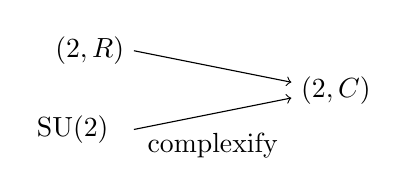
\begin{tikzpicture}
      \node[left] at (0,0.5) {$\SL(2, \mathbb{R})$};
      \node[left] at (-0.2,-0.5) {SU$(2)$};
      \node[right] at (2,0) {$\SL(2,\mathbb{C})$};
      \draw[->] (0,0.5)--(2,0.1);
      \draw[->] (0,-0.5)--(2,-0.1);
      \node at (1,-0.7) {complexify};
    \end{tikzpicture}
  \end{center}
  We can interpret the "real forms" of $\SL(2, \mathbb{C})$ as "slices" of some complex group. However, this does not mean that the real version of these groups are equal. That is, 
  \begin{equation}
    \SL(2, \mathbb{R}) \neq \text{SU}(2)
  \end{equation}

\subsubsection{Lie Algebra of SO(3)}

  It is easy to see that for SO$(2)$, it is easy to see that its Lie algebra $\mathfrak{so}(2)$ has 
  \begin{equation}
    \bigg\{ \begin{pmatrix}
    0&-1\\1&0
    \end{pmatrix}\bigg\}
  \end{equation}
  as its only basis, since 
  \begin{equation}
    exp  \bigg( \begin{pmatrix}
    0&-1\\1&0
    \end{pmatrix} \theta \bigg) = \begin{pmatrix}
    \cos{\theta} & - \sin{\theta} \\
    \sin{\theta} & \cos{\theta}
    \end{pmatrix}
  \end{equation}
  meaning that the dimension of SO$(2)$ is $1$. By adding a component, we can get a rotation in $\mathbb{R}^3$. 
  \begin{align*}
    & R_x = \begin{pmatrix}0&0&0\\0&0&-1\\0&1&0\end{pmatrix} \implies e^{R_x} = \begin{pmatrix}
    1&0&0\\ 0&\cos{\theta}&-\sin{\theta}\\0&\sin{\theta}&\cos{\theta}
    \end{pmatrix}\\
    & R_y = \begin{pmatrix}0&0&1\\0&0&0\\-1&0&0\end{pmatrix} \implies e^{R_y} = \begin{pmatrix}
    \cos{\theta} & 0 & -\sin{\theta}\\ 0&1&0 \\
    \sin{\theta}& 0 & \cos{\theta} \end{pmatrix} \\
    & R_z = \begin{pmatrix}0&-1&0\\1&0&0\\0&0&0\end{pmatrix} \implies e^{R_z} = \begin{pmatrix}
    \cos{\theta} & -\sin{\theta} & 0\\
    \sin{\theta}& \cos{\theta} & 0 \\ 0 & 0 & 1\end{pmatrix}
  \end{align*}
  That is, $e^{R_x}, e^{R_y}$, and $e^{R_z}$ generates a rotation around the $x, y$, and $z$ axis, respectively, which completely generates the group SO$(3)$. Therefore, the Lie algebra $\mathfrak{so}(3)$ consists of the basis 
  \begin{equation}
    \{R_x, R_y, R_z\}
  \end{equation}
  The bracket structure (again, defined as the commutator) of this Lie algebra is 
  \begin{align*}
    & [R_x, R_y] = R_z \\
    & [R_y, R_z] = R_x \\
    & [R_z, R_x] = R_y
  \end{align*}
  which is similar to the brakcet structure of $\mathfrak{su}(2)$. Therefore, SO$(3)$ and SU$(2)$ have the \textbf{same} Lie algebra, which is the algebra of dimension 3 with the same bracket structure. Note that Lie algebras are uniquely determined by the bracket structure and dimension. However, having the same Lie algebra does not imply that the groups are identical (obviously) nor isomorphic. For example, 
  \begin{equation}
    exp(2\pi R_z) = \begin{pmatrix}
    \cos{2\pi} & -\sin{2\pi} & 0 \\
    \sin{2\pi} & \cos{2\pi} & 0 \\
    0 & 0 & 1
    \end{pmatrix} = I
  \end{equation}
  while 
  \begin{equation}
    exp(2\pi A_z) = 
    exp(-i \pi \sigma_z) = exp \bigg(-i \pi \begin{pmatrix}
    1&0\\0&-1
    \end{pmatrix} \bigg) = -I
  \end{equation}
  There is discrepancy by a factor of $-1$. In fact, it turns out that
  \begin{equation}
    \text{SO}(3) = \frac{\text{SU}(2)}{\pm I}
  \end{equation}
  We justify this in the following way. Let $v \in \mathbb{R}^3$ have components $(x, y, z)$. Consider
  \begin{equation}
    M = x \sigma_x + y \sigma_y + z \sigma_z
  \end{equation}
  $M$ is clearly traceless and $M^\dagger = M$. Now, let $S \in$ SU$(2)$ and let $M^\prime = S^{-1} M S$. Then, $\Tr{M^\prime} = \Tr{S^{-1} M S} = \Tr{M} = 0$ and $(M^\prime)^\dagger = (S^{-1} M S)^\dagger = S^\dagger M^\dagger (S^{-1})^\dagger = S^{-1} M S = M^\prime$. Therefore, since $M^\prime$ is self adjoint and traceless, it can be expressed in the form
  \begin{equation}
    x^\prime \sigma_x + y^\prime \sigma_y + z^\prime \sigma_z
  \end{equation}
  for some $(x^\prime, y^\prime, z^\prime)$. Now, since 
  \begin{equation}
    M^2 = (-x^2 - y^2 - z^2) I
  \end{equation}
  we have 
  \begin{align*}
    (M^\prime)^2 & = S^{-1} M^2 S = (-x^2 - y^2 - z^2) I \\
    & = (-x^{\prime 2} - y^{\prime 2} - z^{\prime 2}) I 
  \end{align*}
  So, $x^2 + y^2 + z^2 = x^{\prime 2} + y^{\prime 2} + z^{\prime 2}$, implying that the lengths of $v$ stayed the same. (The proof of linearity of $S$ is easy.) Therefore, the transformation $M \mapsto M^\prime$, i.e. $(x, y, z) \mapsto (x^\prime, y^\prime, z^\prime)$ is a linear transformation preserving length in $\mathbb{R}^3$ (with respect to the usual inner product and norm) $\implies$ it is in SO$(3)$. If we have
  \begin{equation}
    S  = \begin{pmatrix}
    -1&0\\0&-1
    \end{pmatrix}
  \end{equation}
  then $M^\prime = M$, which explains why SO$(3)$ is a coset deviating by both $I$ and $-I$. Visually, if we let SU$(2)$ be a circle, points that are diametrically opposite of each other are "equivalent" in SO$(3)$. That is, SU$(2)$ is a three-dimensional sphere, and $g$ and $-g$ are identified onto the same element in SO$(3)$. This map
  \begin{equation}
    \rho: \text{SU}(2) \rightarrow \text{SO}(3)
  \end{equation}
  in which 2 points are mapped to 1 point is a surjective map with
  \begin{equation}
    \ker{\rho} = \{I, -I\}
  \end{equation}
  \begin{center}
    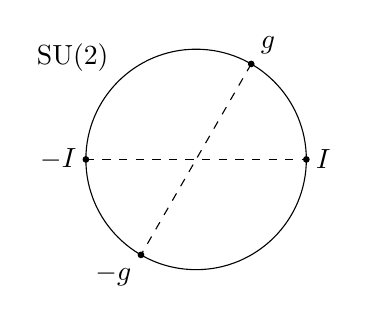
\begin{tikzpicture}[scale=0.7]
      \draw (0,0) circle (2);
      \draw[fill] (2,0) circle (0.05);
      \draw[fill] (-2,0) circle (0.05);
      \node[right] at (2,0) {$I$};
      \node[left] at (-2,0) {$-I$};
      \draw[fill] (1,1.732) circle (0.05);
      \draw[fill] (-1,-1.732) circle (0.05);
      \node[above right] at (1, 1.732) {$g$};
      \node[below left] at (-1, -1.732) {$-g$};
      \draw[dashed] (-2,0)--(2,0);
      \draw[dashed] (1, 1.732)--(-1, -1.732);
      \node[above left] at (-1.414, 1.414) {SU$(2)$};
    \end{tikzpicture}
  \end{center}

  We can in fact explicitly describe exponential map from $\mathfrak{so}(3)$ to SO$(3)$ with the following lemma. 

  \begin{lemma}[Rodrigues' Formula]
    The exponential map $exp: \mathfrak{so}(3) \rightarrow$ SO$(3)$ is defined by 
    \begin{equation}
      e^A = \cos{\theta} I_3 + \frac{\sin{\theta}}{\theta} A + \frac{(1 - \cos{\theta})}{\theta^2} B
    \end{equation}
    where 
    \begin{equation}
      A = \begin{pmatrix}
      0&-c&b\\c&0&-a\\-b&a&0
      \end{pmatrix}, B = \begin{pmatrix}
      a^2&ab&ac\\ab&b^2&bc\\ac&bc&c^2
      \end{pmatrix}
    \end{equation}
    This formula has many applications in kinematics, robotics, and motion interpolation. 
  \end{lemma}

  \begin{theorem}
  The Lie algebras for the following classical Lie groups are summarized as follows. 
  \begin{enumerate}
    \item $\mathfrak{sl}_n \mathbb{R}$ is the real vector space of real $n \times n$ matrices with null trace.
    \item $\mathfrak{so}(n)$ is the real vector space of real $n \times n$ skew-symmetric matrices. 
    \item $\mathfrak{gl}_n \mathbb{R}$ is the real vector space of all real $n \times n$ matrices.
    \item $\mathfrak{o}(n) = \mathfrak{o}(n)$
  \end{enumerate}
  \end{theorem}
  Note that the corresponding groups $\GL(n, \mathbb{R}), \SL(n, \mathbb{R}), \mathfrak{gl}_n \mathbb{R}, \mathfrak{sl}_n \mathbb{R}$ are Lie groups, meaning that they are smooth real manifolds. We can view each of them as smooth real manifolds embedded in the $n^2$ dimensional vector space of real matrices, which is isomorphic to $\mathbb{R}^{n^2}$. 

  \begin{theorem}
    The Lie algebras $\mathfrak{gl}_ \mathbb{R}, \mathfrak{sl}_n \mathbb{R}, \mathfrak{o}(n), \mathfrak{so}(n)$ are well-defined, but only 
    \begin{equation}
      exp: \mathfrak{so}(n) \rightarrow \text{SO}(n)
    \end{equation}
    is surjective. 
  \end{theorem}

  \begin{theorem}
    The Lie algebras for the following classical Lie groups are summarized as follows. 
    \begin{enumerate}
      \item $\mathfrak{sl}_2 \mathbb{C}$ is the real (or complex) vector space of traceless complex $n \times n$ matrices. 
      \item $\mathfrak{u}(n)$ is the real vector space of complex $n \times n$ skew-Hermitian matrices. 
      \item $\mathfrak{su}(n) = \mathfrak{u} \cap \mathfrak{sl}_2 \mathbb{C}$. It is also a real vector space. 
      \item $\mathfrak{gl}_n \mathbb{C}$ is the real (or complex) vector space of complex $n \times n$ matrices. 
    \end{enumerate}
    Note that even though the matrices in these Lie algebras have complex coefficients, we have assigned them to be in a \textbf{real} vector space, which means that we are only allowed to take real linear combinations of these elements. That is, the field we are working over is $\mathbb{R}$ (this does not contradict any of the axioms for vector spaces). For example an element $A$ in $\mathfrak{u}(n)$ or $\mathfrak{su}(n)$ must be anti-self adjoint, but $iA$ is self adjoint. 
  \end{theorem}

  Similarly, the Lie groups 
  \begin{equation}
    \GL(n, \mathbb{C}), \SL(n, \mathbb{C}), \mathfrak{gl}_n \mathbb{C}, \mathfrak{sl}_n \mathbb{C}
  \end{equation}
  are also smooth real manifolds embedded in Mat$(n, \mathbb{C}) \simeq \mathbb{C}^{n^2} \simeq \mathbb{R}^{2 n^2}$. So, we can view these four groups as manifolds embedded in $\mathbb{R}^{2 n^2}$. 

  Note some of the similarities and differences between the real and complex counterparts of these Lie groups and algebras. 
  \begin{enumerate}
    \item $\mathfrak{o}(n) = \mathfrak{so}(n)$, but $\mathfrak{u}(n) \neq \mathfrak{su}(n)$. 
    \item $exp: \mathfrak{gl}_n \mathbb{R} \rightarrow \GL(n, \mathbb{R})$ is not surjective, but $exp: \mathfrak{gl}_n \mathbb{C} \rightarrow \GL(n, \mathbb{C})$ is surjective due to the spectral theorem and surjectivity of $exp: \mathbb{C} \rightarrow \mathbb{C}^*$.
    \item The exponential maps $exp: \mathfrak{u}(n) \rightarrow \text{U}(n)$ and $exp: \mathfrak{su}(n) \rightarrow \text{SU}(n)$ are surjective. 
    \item Still, $exp: \mathfrak{sl}_2 \mathbb{C} \rightarrow \SL(2, \mathbb{C})$ is not surjective. This will be proved now. 
  \end{enumerate}

  \begin{theorem}
    $exp: \mathfrak{sl}_2 \mathbb{C} \rightarrow \SL(2, \mathbb{C})$ is not surjective. 
  \end{theorem}
  \begin{proof}
    Given $M \in \SL(n, \mathbb{C})$, assume that $M = e^A$ for some matrix $A \in \mathfrak{sl}_2 \mathbb{C}$. Putting $A$ into the Jordan Normal Form $J = N A N^{-1}$ means that $J$ can either be of form
    \begin{equation}
      J = \begin{pmatrix}
      0&1\\0&0
      \end{pmatrix}, \begin{pmatrix}
      \lambda&0\\0&-\lambda
      \end{pmatrix} \implies e^J = \begin{pmatrix}
      1&1\\0&1
      \end{pmatrix}, \begin{pmatrix}
      e^\lambda&0\\0&e^{-\lambda}
      \end{pmatrix}
    \end{equation}
    which is also in JNF in $\SL(2, \mathbb{C})$. But a matrix $P \in \SL(2, \mathbb{C})$ may exist with JNF of 
    \begin{equation}
      K = \begin{pmatrix}
      -1&1\\0&-1
      \end{pmatrix}
    \end{equation}
    which is not one of the 2 forms. So, $K \not\in \im{exp} \implies exp$ is not surjective. 
  \end{proof}

  \begin{theorem}
  The exponential maps 
  \begin{align*}
    & exp: \mathfrak{u}(n) \rightarrow \text{U}(n) \\
    & exp: \mathfrak{su}(n) \rightarrow \text{SU}(n)
  \end{align*}
  are surjective. 
  \end{theorem}

\subsubsection{Lie Algebra of SE(n)}

  Recall that the group of affine rigid isometries is denoted SE$(n)$. That is, 
  \begin{equation}
    \text{SE}(n) \equiv \text{SO}(n) \ltimes \text{Tran}\,\mathbb{R}^n
  \end{equation}
  We can define the matrix representation of this affine transformation as such. Given an element $g \in$ SE$(n)$ such that
  \begin{equation}
    g(x) \equiv R x + U, \; R \in \text{SO}(n), U \in \text{Tran}\, \mathbb{R}^n 
  \end{equation}
  we define the representation
  \begin{equation}
    \rho: \text{SE}(n) \rightarrow \GL(n+1, \mathbb{R}), \rho(g) \equiv \begin{pmatrix}
    R&U\\0&1
    \end{pmatrix}
  \end{equation}
  where $R$ is a real $n\times n$ matrix in SO$(n)$ and $U$ is a real $n$-vector in Tran$\,\mathbb{R}^n \simeq \mathbb{R}^n$. We would then have
  \begin{equation}
    \rho(g) \begin{pmatrix}
    x\\1
    \end{pmatrix} \equiv \begin{pmatrix}
    R&U\\0&1
    \end{pmatrix} \begin{pmatrix}
    x\\1
    \end{pmatrix} = \begin{pmatrix}
    R x + U\\1
    \end{pmatrix} \in \mathbb{R}^{n+1}
  \end{equation}

  Clearly, SE$(n)$ is a Lie group, and the matrix representation $\varrho$ of its Lie algebra $\mathfrak{se}(n)$ can be defined as the vector space of $(n+1) \times (n+1)$ matrices of the block form 
  \begin{equation}
    A = \begin{pmatrix}
    \Omega & U \\0 & 0
    \end{pmatrix}
  \end{equation}
  where $\Omega$ is an $n \times n$ skew-symmetric matrix and $U \in \mathbb{R}^n$. Note that there are two different exponential maps here: one belonging to the abstract Lie group SE$(n)$ and another belonging to the concrete, matrix group $\GL(n+1, \mathbb{R})$. This can be represented with the commutative diagram. 
  \[\begin{tikzcd}
  \mathfrak{se}(n) \arrow{r}{exp} \arrow{d}{\varrho} & SE(n) \arrow{d} {\rho}\\
  \mathfrak{gl}_{n+1} \mathbb{R} \arrow{r}{exp} & \GL(n+1, \mathbb{R})
  \end{tikzcd}\]

  \begin{lemma}
    Given any $(n+1) \times (n+1)$ matrix of form 
    \begin{equation}
      A = \begin{pmatrix}
       \Omega & U \\0&0
      \end{pmatrix}
    \end{equation}
    where $\Omega$ is any matrix and $U \in \mathbb{R}^n$, 
    \begin{equation}
      A^k = \begin{pmatrix}
      \Omega^k & \Omega^{k-1} U \\0&0
      \end{pmatrix}
    \end{equation}
    where $\Omega^0 = I_n$, which implies that
    \begin{equation}
      e^A = \begin{pmatrix}
      e^\Omega & V U \\ 0 & 1
      \end{pmatrix}, \; V = I_n + \sum_{k \geq 1} \frac{\Omega^k}{(k+1)!}
    \end{equation}
  \end{lemma}

  \begin{theorem}
    The exponential map
    \begin{equation}
      exp: \mathfrak{se}(n) \rightarrow SE(n)
    \end{equation}
    is well-defined and surjective. 
  \end{theorem}

\subsection{Representations of Lie Groups and Lie Algebras}

  Let $\mathcal{G}$ be an abstract group and let
  \begin{equation}
    \rho: \mathcal{G} \rightarrow \GL(V)
  \end{equation}
  be the representation of $\mathcal{G}$. Then, let $\mathfrak{g}$ be the Lie algebra of $\mathcal{G}$, and $\mathfrak{gl}(V)$ be the Lie algebra of $\GL(V)$. Then, $\rho$ induces another homomorphism 
  \begin{equation}
    \varrho: \mathfrak{g} \rightarrow \mathfrak{gl}(V)
  \end{equation}
  where the bracket structure (in this case, the comutator in the matrix algebra) is preserved. 
  \begin{equation}
    \varrho([X,Y]) = [\varrho(X), \varrho(Y)]
  \end{equation}
  We can visualize this induced homomorphism with the following commutative diagram, which states that $\rho \circ exp = exp \circ \varrho$. 

  \[\begin{tikzcd}
  \mathcal{G} \arrow{r}{\rho} & \GL(V)\\
  \mathfrak{g} \arrow{u}{exp} \arrow{r}{\varrho} & \mathfrak{gl}(V) \arrow{u}{exp}
  \end{tikzcd}\]

  Note that there are very crucial differences between $\rho$ and $\varrho$. First, $\rho$ is a homomorphism between \textbf{groups}, while $\varrho$ is a homomorphism between \textbf{vector spaces}. Additionally, $\GL(V)$ is a group, not a linear space, while $\mathfrak{gl}(V)$ is a linear space. Finally, note that $\GL(V)$ is restricted to only matrices with nonzero determinants, while the elements of $\mathfrak{gl}(V)$ can be any matrix. 

  \begin{example}
    The representation of SE$(n)$ to $\GL(n+1 \mathbb{R}$ and $\mathfrak{se}(n)$ to $\mathfrak{gl}_{n+1} \mathbb{R}$ induces the second homomorphism $\varrho: \mathfrak{gl}_{n+1} \mathbb{R} \rightarrow \GL(n+1, \mathbb{R})$. 
  \end{example}

  \begin{definition}
    The direct sum of representations is a representation. That is, if $U$ is a representation and $V$ is a representation, then $U \oplus V$ is a representation. That is, if 
    \begin{equation}
      \rho_1: \mathcal{G} \rightarrow U, \; \rho_1 (g) = \begin{pmatrix}
      u_1&u_2\\u_3&u_4
      \end{pmatrix}
    \end{equation}
    and
    \begin{equation}
      \rho_2: \mathcal{G} \rightarrow V, \; \rho_2 (g) = \begin{pmatrix}
      v_1 & v_2 \\ v_3 & v_4
      \end{pmatrix}
    \end{equation}
    are two representations of the same group element $g \in \mathcal{G}$, then 
    \begin{equation}
      (\rho_1 \oplus \rho_2): \mathcal{G} \rightarrow (U \oplus V), \;(\rho_1 \oplus \rho_2) (g) = \begin{pmatrix}
      u_1 & u_2 & 0 & 0 \\
      u_3 & u_4 & 0 & 0 \\
      0 & 0 & v_1 & v_2 \\
      0 & 0 & v_3 & v_4 
      \end{pmatrix}
    \end{equation}
    is a bigger representation of $g$ in $U \oplus V$. 
  \end{definition}

  \begin{definition}
    $V$ is irreducible if the only subspaces which are representations are only $V$ and $\{0\}$. 
  \end{definition}

  For our case, we will consider that any representation can be written as a direct sum of irreducible representations. We will now proceed to find an irreducible representation of $\mathfrak{sl}_2 \mathbb{C}$. This means that we want to find the smallest (lowest dimensional) vector space $V$ such that there exists a representation
  \begin{equation}
    \varrho: \mathfrak{sl}_2 \mathbb{C} \rightarrow \mathfrak{gl}(V)
  \end{equation}
  We will write, as shorthand notation, that 
  \begin{equation}
    H = \varrho(H), X = \varrho(X), Y = \varrho(Y)
  \end{equation}
  Clearly, $H, X, Y \in \mathfrak{gl}(V) \simeq \mathfrak{gl}(\mathbb{C}^n)$. By the spectral theorem, we can find an orthonormal basis of eigenvectors $e_1, e_2, ..., e_n$ of the mapping $H$ such that
  \begin{equation}
    H e_i = \lambda_i e_i, \; \lambda_i \in \mathbb{C}
  \end{equation}
  Since $[H,X] = 2X$, it follows that $HX e_i - X H e_i = 2X e_i \implies H (X e_i) = (\lambda_i + 2) (X e_i) \implies Xe_i$ for all $i = 1, 2, ..., n$ are also eigenvectors of $H$ with eigenvalue $(\lambda_i + 2)$, or $X e_i = 0$. So, $X$ is a "ladder operator" that maps each eigenvector $e_i$ with eigenvalue $\lambda_i$ to a different eigenvector $e_j$ with eigenvalue $\lambda_j = \lambda_i + 2$. Having nowhere to be mapped to, the eigenvector with the largest eigenvalue (which must exist since $V$ is finite dimensional) will get mapped to the $0$ vector by $X$. Let us denote this eigenvector having the maximum eigenvalue $m$, as $v_m$. 

  Similarly, $[H,Y] = -2Y$ implies that
  \begin{equation}
    HY e_i - YH e_i = -2Y e_i \implies H(Y e_i) = (\lambda_i - 2)(Y e_i)
  \end{equation}

  implying that $Y$ maps each eigenvector $e_i$ with eigenvaue $\lambda_i$ to another eigenvector $e_j$ with eigenvalue $\lambda_j = \lambda_i - 2$, except for the eigenvector with smallest eigenvalue, which gets mapped to $0$. Since $Y$ clearly maps each eigenvector to a different eigenvector that has a strictly decreasing eigenvalue, we can construct a basis of $V$ to be
  \begin{equation}
    \{v_m, Y v_m, Y^2 v_m, Y^3 v_m, ..., Y^{n-1} v_m\}
  \end{equation}
  (remember that $Y^n v_m = 0$). So, elements of $\mathfrak{sl}_2 \mathbb{C}$ acts on the space $V$ with basis above. To continue, we introduce the following theorem. 

  \begin{theorem}
    \begin{equation}
      X Y^j v_m = j(m-j+1) Y^{j-1} v_m
    \end{equation}
  \end{theorem}
  \begin{proof}
    By induction on $j$ using bracket relations.
  \end{proof}

  $V$ is $n$-dimensional. Since $Y^n v_m = 0$ and $Y^{n-1} v_m \neq 0$, we use the theorem above to get
  \begin{equation}
    0 = X Y^n v_m = n (m-n+1) Y^{n-1} v_m \implies m-n+1=0
  \end{equation}
  So, $n = m+1$, which means that the eigenvalues of $H$ are
  \begin{equation}
    m, m-2, m-4, \ldots, m - 2(n-1) = -m
  \end{equation}

  and we are done. We now classify the 1, 2, and 3 dimensional irreducible representations of $\mathfrak{sl}_2 \mathbb{C}$. 
  \begin{enumerate}
    \item When $n = 1$ (i.e. dimension is 1), $m = n-1 = 0$, meaning that the greatest (and only) eigenvalue is $0$. That is, 
      \begin{equation}
        H v_0 = 0,\; X v_0 = 0,\; Y v_0 = 0
      \end{equation}
    which is the trivial representation of $\mathfrak{sl}_2 \mathbb{C}$. Explicitly, we can completely define the representation (which is a linear homomorphism) with the three equations. 
    \begin{equation}
      \varrho(H) = (0),\; \varrho(X) = (0),\; \varrho(Y) = (0)
    \end{equation}

    \item When $n = 2$ and $m=1$. We now look for a 2 dimensional irreducible representation. The eigenvalues are $1$ and $-1$, with $\{v_1, v_{-1}\}$ as a basis of 2 dimensional space $V$. Then we have 
      \begin{align*}
        & Hv_1 = v_1, \; Hv_{-1} = - v_{-1} \\
        & X v_1 = 0, \; X v_{-1} = v_1 \\
        & Y v_1 = v_{-1}, \; Y v_{-1} = 0
      \end{align*}
    which explicitly translates to the representation $\varrho$ being defined
    \begin{equation}
      \varrho(H) = \begin{pmatrix}
      1&0\\0&-1
      \end{pmatrix}, \; \begin{pmatrix}
      0&1\\0&0
      \end{pmatrix}, \; \begin{pmatrix}
      0&0\\1&0
      \end{pmatrix}
    \end{equation}

    \item When $n=3 \implies m=2$, the basis is $\{v_{-2}, v_0, v_2\}$ with eigenvalues $2, 0, -2$, and the irreducible representation $\varrho$ is defined
      \begin{equation}
        \varrho(H) = \begin{pmatrix}
        2&&\\&0&\\&&-2
        \end{pmatrix}, \varrho(Y) = \begin{pmatrix}
        0&0&0\\1&0&0\\0&1&0
        \end{pmatrix}, \varrho(X) = \begin{pmatrix}
        0&1&0\\0&0&1\\0&0&0
        \end{pmatrix}
      \end{equation}

    \item The same process continues on for $n=4, 5, ...$, and this entirely classifies the irreducible representations of $\mathfrak{sl}_2 \mathbb{C}$. 
  \end{enumerate} 

  \pagebreak

  \subsubsection{Tensor Products of Group Representations}

    \begin{definition}
      If $V$ and $W$ are two different representations of a group $\mathcal{G}$, then we know that $V \oplus W$ is also a representation of $\mathcal{G}$. Furthermore, the tensor product space $V \otimes W$ also defines a representation of $\mathcal{G}$. That is, given representations
      \begin{align*}
        & \rho_V: \mathcal{G} \rightarrow \GL(V) \\
        & \rho_W: \mathcal{G} \rightarrow \GL(W)
      \end{align*}
      The homomorphism $\rho_V \otimes \rho_W: \mathcal{G} \rightarrow \GL(V \otimes W)$ is also a representation of $\mathcal{G}$, which is defined
      \begin{equation}
        (\rho_V \otimes \rho_W)(g) (v \otimes w) \equiv \rho_V (g) (v) \otimes \rho_W (g) (w)
      \end{equation}
      or represented in shorthand notation, 
      \begin{equation}
        g(v \otimes w) \equiv (g v) \otimes (g w)
      \end{equation}
      We know that exp$(H)$ acts on $V$ and $W$ since it is an element of $\GL(V)$ and $\GL(W)$. This means that
      \begin{equation}
        exp(H)(v \otimes w) \equiv \big( exp(H)(v)\big) \otimes \big( exp(H)(w)\big)
      \end{equation}
      If $H$ ($= \rho_V (H)$ or $\rho_W(H)$) has an eigenvalue $\lambda$ on $v$ in $V$ and eigenvalue $\mu$ on $w$ in $W$, then 
      \begin{equation}
        exp(H) (v \otimes w) = (e^\lambda v) \otimes (e^\mu w) = e^{\lambda + \mu} v \otimes w
      \end{equation}
      That is, eigenvalues of $H$ \textbf{add} on tensor products. 
    \end{definition}

    \begin{example}
      Recall that the $2$ dimensional representation $V$ of $\mathfrak{sl}_2 \mathbb{C}$ has eigenvalues $1$ and $-1$ (with corresponding eigenvectors $e_1$ and $e_{-1}$). So, $V \otimes V$ has eigenvalues 
      \begin{align*}
        & (-1) + (-1) = -2, \;\; (-1) + 1 = 0 \\
        & 1 + (-1) = 0, \;\; 1 + 1 = 2
      \end{align*}
      Therefore, the eigenvalues of $V \otimes V$ is $-2$ (geometric multiplicity of 1), $0$ (geometric multiplicity of 2), and $2$ (geometric multiplicity of 1), (Notation-wise, the $n$-dimensional irreducible representation of $\mathfrak{sl}_2 \mathbb{C}$ is denoted $\mathbf{n}$.) which means that
      \begin{equation}
        \mathbf{2} \otimes \mathbf{2} = \mathbf{3} \oplus \mathbf{1}
      \end{equation}
      We can decompose $V \otimes V$ into its symmetric and exterior power components. Sym$^2 V$ has basis (of eigenvectors)
      \begin{equation}
        \{e_{-1} \odot e_{-1}, \; e_{-1} \odot e_1, \; e_1 \odot e_1\}
      \end{equation}
      where the corresponding eigenvalues are $-2$, $0$, and $2$, respectively. So, $\dim{Sym^2 V} = 3$, which means that $Sym^2 V = \mathbf{3}$. As for the exterior power component of $V$, $\Lambda^2 V$ has basis $\{e_{-1} \wedge e_1\}$ with eigenvalue $= 0 \implies \dim{\Lambda^2 V} = 1$, meaning that $\Lambda^2 V = \mathbf{1}$. Therefore, 
      \begin{equation}
        V \otimes V = Sym^2 V \oplus \Lambda^2 V = \mathbf{3} \oplus \mathbf{1}
      \end{equation}
    \end{example}

\subsection{Topological Decompositions of Lie Groups}

  \begin{definition}
    Let us define 
    \begin{enumerate}
      \item S$(n)$ is the vector space of real, symmetric $n \times n$ matrices. 
      \item SP$(n)$ is the set of symmetric, positive semidefinite matrices. 
      \item SPD$(n)$ is the set of symmetric, positive definite matrices. 
    \end{enumerate}
    Note that SP$(n)$ and SPD$(n)$ are not even vector spaces at all. 
  \end{definition}

  \begin{lemma}
    The exponential map 
    \begin{equation}
      exp: S(n) \rightarrow SPD(n)
    \end{equation}
    is a homeomorphism. One may be tempted to call S$(n)$ the Lie algebra of SPD$(n)$, but this is not the case. S$(n)$ is not even a Lie algebra since the commutator is not algebraically closed. Furthermore, SPD$(n)$ is not even a multiplicative group (since matrix multiplication is not closed). 
  \end{lemma}

  Recall from linear algebra the Polar Decomposition. We express this result in a slightly modified way. 

  \begin{theorem}[Polar Decomposition]
    Given a Euclidean space $\mathbb{E}^n$ and any linear endomorphism $f$ of $\mathbb{E}^n$, there are two positive definite self-adjoint linear maps $h_1, h_2 \in$ End$(\mathbb{E}^n)$ and $g \in$ O$(n)$ such that
    \begin{equation}
      f = g \circ h_1 = h_2 \circ g
    \end{equation}
    That is, such that $f$ can be decomposed into the following compositions of functions that commute. 

    \[\begin{tikzcd}
    \mathbb{E}^n \arrow{r}{h_2} & \mathbb{E}^n \\
    \mathbb{E}^n \arrow{u}{g} \arrow{ur}{f} \arrow{r}{h_1} & \mathbb{E}^n \arrow{u}{g}
    \end{tikzcd}\]

    This means that there is a bijection between $Mat(n, \mathbb{R})$ and $O(n) \times SP(n)$. If $f$ is an automorphism, then this decomposition is unique. 
  \end{theorem}

  \begin{corollary}
    The two topological groups are homeomorphic. 
    \begin{equation}
      GL(n, \mathbb{R}) \cong O(n) \times SPD(n)
    \end{equation}
  \end{corollary}

  \begin{corollary}
    For every invertible real matrix $A \in GL(n, \mathbb{R})$, there exists a unique orthogonal matrix $R$ and unique symmetric matrix $S$ such that
    \begin{equation}
      A = R e^S
    \end{equation}
    $\implies$ there is a bijection between $\GL(n, \mathbb{R})$ and $O(n) \times S(n) \simeq \mathbb{R}^{n(n+1)/2}$. Moreover, they are homeomorphic. That is, 
    \begin{equation}
      \GL(n, \mathbb{R}) \simeq O(n) \times S(n) \simeq O(n) \times \mathbb{R}^{n(n+1)/2}
    \end{equation}
    This essentially reduces the study of $\GL(n, \mathbb{R})$ to the study of $O(n)$, which is nice since $O(n)$ is compact. 
  \end{corollary}

  \begin{corollary}
    Given a real matrix $A$, if $\det{A} > 0$, then we can decompose $A$ as
    \begin{equation}
      A = R e^S
    \end{equation}
    where $R \in SO(n)$ and $S \in S(n)$. 
  \end{corollary}

  \begin{corollary}
    There exists a bijection between
    \begin{equation}
      \SL(n, \mathbb{R}) \text{ and } SO(n) \times (S(n) \cap \mathfrak{sl}_n \mathbb{R})
    \end{equation}
  \end{corollary}
  \begin{proof}
    $A \in \SL(n, \mathbb{R}) \implies 1 = \det{A} = \det{R} \det{e^S} = \det{e^S} \implies \det{e^S} = e^{\Tr{S}} = 1 \implies \Tr{S} = 0 \implies S \in$ S$(n) \cap \mathfrak{sl}_n \mathbb{R}$. 
  \end{proof}

  \begin{definition}
    Let us define
    \begin{enumerate}
      \item H$(n)$ is the real vector space of $n \times n$ Hermitian matrices. 
      \item HP$(n)$ is the set of Hermitian, positive semidefinite $n \times n$ matrices. 
      \item HPD$(n)$ is the set of Hermitian, positive definite $n \times n$ matrices. 
    \end{enumerate}
    Similarly, HP$(n)$ and HPD$(n)$ are not vector space. They are just sets. 
  \end{definition}

  \begin{lemma}
    The exponential mapping
    \begin{equation}
      exp: H(n) \rightarrow HPD(n)
    \end{equation}
    is a homeomorphism. 
  \end{lemma}

  However again, HPD$(n)$ is not a Lie group (multiplication is not algebraically closed) nor is H$(n)$ a Lie algebra (commutator is not algebraically closed). By the polar form theorem of complex $n \times n$ matrices, we have a (not necessarily unique) bijection between
  \begin{equation}
    \text{Mat}(n, \mathbb{C}) \text{ and } U(n) \times HP(n)
  \end{equation}
  which implies that
  \begin{equation}
    \GL(n, \mathbb{C}) \cong U(n) \times HPD (n)
  \end{equation}

  \begin{corollary}
    For every complex invertible matrix $A$, there exists a unique decomposition
    \begin{equation}
      A = U e^S
    \end{equation}
    where $U \in U(n)$ and $S \in H(n)$, which implies that the following groups are homeomorphic. 
    \begin{align*}
      \GL(n, \mathbb{C}) & \cong U(n) \times H(n) \\
      & \cong U(n) \times \mathbb{R}^{n^2}
    \end{align*} 
    This essentially reduces the study of $\GL(n, \mathbb{C})$ to that of U$(n)$. 
  \end{corollary}

  \begin{corollary}
    There exists a bijection between 
    \begin{equation}
      \SL(n, \mathbb{C}) \text{ and } SU(n) \times (H(n) \cap \mathfrak{sl}_n \mathbb{C})
    \end{equation}
  \end{corollary}
  \begin{proof}
    Similarly, when $A = U e^S$, we know that $|\det{U}| = 1$ and $\Tr{S}$ is real (since by the Spectral theorem, every self adjoint matrix has a real spectral decomposition). Since $S$ is Hermitian, this implies that $\det{e^S} > 0$. If $A \in \SL(n, \mathbb{C})$, then $\det{A} = 1 \implies \det{e^S} = 1 \implies S \in H(n) \cap \mathfrak{sl}_n \mathbb{C}$. 
  \end{proof}

\subsection{Linear Lie Groups}

  We will assume that the reader has the necessary background knowledge in manifolds, chart mappings, diffeomorphisms, tangent spaces, and transition mappings. 

  Recall that the algebra of real $n \times n$ matrices Mat$(n, \mathbb{R})$ is bijective to $\mathbb{R}^{n^2}$, which is a topological space. Therefore, this bijection 
  \begin{equation}
    i:(\mathbb{R}^{n^2}, \tau_E) \rightarrow \text{Mat}(n, \mathbb{R})
  \end{equation}
  induces a topology on Mat$(n, \mathbb{R})$, defined 
  \begin{equation}
    \tau_M \equiv \{U \in \text{Mat}(n, \mathbb{R}) \; | \; e^{-1} (U) \in \tau_E\}
  \end{equation}
  With this, consider the subset
  \begin{equation}
    \GL(n, \mathbb{R}) \subset \text{Mat}(n, \mathbb{R})
  \end{equation}
  where
  \begin{equation}
    \GL(n, \mathbb{R}) \equiv \{x \in \text{Mat}(n, \mathbb{R}) \;|\; \det{x} \neq 0\}
  \end{equation}
  This set, as we expect, is a multiplicative group. 

  \begin{definition}
    The \textbf{general linear group}, denoted $\GL(n, \mathbb{R})$ is the set of $n \times n$ matrices with nonzero determinant. The more technical definition is that $\GL(n, \mathbb{R})$ is really just the automorphism group of $\mathbb{R}^n$, 
    \begin{equation}
      \GL(n, \mathbb{R}) \equiv \text{Aut}(\mathbb{R}^n)
    \end{equation}
    but it is customary to assume a basis on $\mathbb{R}^n$ in order to realize $\GL(n, \mathbb{R})$ as a matrix group. Note that the procedure of assuming a basis on $\mathbb{R}^n$ is the same as defining a representation of the abstract group $\GL(n, \mathbb{R})$. Both assigns a real $n \times n$ matrix to each element of $\GL(n, \mathbb{R})$. 
  \end{definition}

  In this way, we can view $\GL(n, \mathbb{R})$ as a topological space in $\mathbb{R}^{n^2}$, and it is fine to interpret $\GL(n, \mathbb{R})$ as a matrix group rather than an abstract group. 

  Since the matrix representation of $\GL(n, \mathbb{R})$ is always well defined, the abstract subgroups of $\GL(n, \mathbb{R})$, which are $\SL(n, \mathbb{R}), O(n)$, and $SO(n)$, also have well defined matrix representations (that we are all familiar with). Additionally, since there exists a bijection
  \begin{equation}
    \text{Mat}(n, \mathbb{C}) \cong \mathbb{C}^{n^2} \cong \mathbb{R}^{2 n^2}
  \end{equation}
  we can view $\GL(n, \mathbb{C})$ as a subset of $\mathbb{R}^{2n^2}$, meaning that the subgroups $\SL(n, \mathbb{C}), U(n)$, and $SU(n)$ of $\GL(n, \mathbb{C})$ can also be viewed as subsets of $\mathbb{R}^{2n^2}$. This also applies to $SE(n)$ since it is a subgroup of $\SL(n+1, \mathbb{R})$. We formally state it now. 

  \begin{theorem}
    SE$(n)$ is a linear Lie group. 
  \end{theorem}
  \begin{proof}
    The matrix representation of elements $g \in SE(n)$ is 
    \begin{equation}
      \rho(g) \equiv \begin{pmatrix}
      R_g & U_g \\ 0 & 1
      \end{pmatrix}, \; R_g \in SO(n), U_g \in \mathbb{R}^n
    \end{equation}
    But such matrices also belong to the bigger group $\SL(n+1, \mathbb{R}) \implies SE(n) \subset \SL(n+1, \mathbb{R})$. Moreover, this canonical embedding 
    \begin{equation}
      i: SE(n) \rightarrow \SL(n+1, \mathbb{R})
    \end{equation}
    is a group homomorphism since
    \begin{align*}
      i\big( \rho(g_1 \cdot g_2) \big) & = \begin{pmatrix}
      RS & RV + U \\ 0 & 1
      \end{pmatrix} \\
      & = \begin{pmatrix}
      R & U \\ 0 & 1
      \end{pmatrix} \begin{pmatrix}
      S & V \\ 0 & 1
      \end{pmatrix} = \rho \big( i(g_1) \cdot i(g_2) \big) 
    \end{align*}
    and the inverse is given by 
    \begin{equation}
      \begin{pmatrix}
      R & U \\ 0 & 1
      \end{pmatrix}^{-1} = \begin{pmatrix}
      R^{-1} & - R^{-1} U \\ 0 & 1
      \end{pmatrix} = \begin{pmatrix}
      R^T & - R^T U \\ 0 & 1
      \end{pmatrix}
    \end{equation}
    is also consistent between the inverse operation in SE$(n)$ and $\SL(n+1, \mathbb{R})$. Therefore, SE$(n)$ is a subgroup of $\SL(n+1, \mathbb{R})$, which is a subgroup of $\GL(n+1, \mathbb{R})$. 
  \end{proof}

  Note that even though SE$(n)$ is diffeomorphic (a topological relation) to SO$(n) \times \mathbb{R}^n$, it is \textbf{not} isomorphic (an algebraic relation) sicne group operations are not preserved. Therefore, we write this "equality" as a semidirect product of groups. 
  \begin{equation}
    SE(n) \equiv SO(n) \ltimes \mathbb{R}^n
  \end{equation}

  Therefore, all of the classical Lie groups that we have mentioned can be viewed as subsets of $\mathbb{R}^N$ (with the subspace topology) and as subgroups of $\GL(N, \mathbb{R})$ for some big enough $N$. This defines a special family of Lie groups, called linear Lie groups. 

  \begin{definition}
    A \textbf{linear Lie group} is a subgroup of $\GL(n, \mathbb{R})$ for some $n \geq 1$ which is also a smooth manifold in $\mathbb{R}^{n^2}$. 
  \end{definition}

  \begin{theorem}[Von Neumann, Cartan]
    A closed subgroup $\mathcal{G}$ of $\GL(n, \mathbb{R})$ is a linear Lie group. That is, a closed subgroup $\mathcal{G}$ of $\GL(n, \mathbb{R})$ is a smooth manifold in $\mathbb{R}^{n^2}$.
  \end{theorem}

  \begin{definition}
    Since a linear Lie group $\mathcal{G}$ is a smooth submanifold in $\mathbb{R}^N$, we can take its tangent space at the identity element $I$, which is defined 
    \begin{equation}
      T_I \mathcal{G} \equiv \{p^\prime (0) \;|\; p: I \subset \mathbb{R} \rightarrow \mathcal{G}, p(0) = I\}
    \end{equation}
    where $p$ is a path function on $\mathcal{G}$. 
  \end{definition}

  Note that we haven't mentioned anything about the exponential map up to now. We mention the relationship between this map and the Lie algebra with the following theorem. 

  \begin{theorem}
    Let $\mathcal{G}$ be a linear Lie group. The set $\mathfrak{g}$ defined such that
    \begin{equation}
      \mathfrak{g} \equiv \{X \in \text{Mat}(n, \mathbb{R}) \; | \; e^{t X} \in \mathcal{G} \; \forall t \in \mathbb{R}\}
    \end{equation}
    is equal to the tangent space of $\mathcal{G}$ at the identity element. That is, 
    \begin{equation}
      \mathfrak{g} = T_I \mathcal{G}
    \end{equation}
    Furthermore, $\mathfrak{g}$ is closed under the commutator 
    \begin{equation}
      [A,B] \equiv A B - B A
    \end{equation}
  \end{theorem}

  This theorem ensures that given a linear Lie group $\mathcal{G}$, the tangent space $\mathfrak{g}$ exists and is closed under the commutator. We formally define this space. 

  \begin{definition}
    The Lie algebra of a linear Lie group is a real vector space (of matrices) together with a algebraically closed bilinear map 
    \begin{equation}
      [A,B] \equiv A B - B A
    \end{equation}
    called the \textbf{commutator}. 
  \end{definition} 

  The definition of $\mathfrak{g}$ given in the previous theorem shows that 
  \begin{equation}
    exp: \mathfrak{g} \rightarrow \mathcal{G}
  \end{equation}
  is well defined. In general, exp is neither injective nor surjective. Visually, this exponential mapping is what connects the Lie algebra, i.e. the tangent space of manifold $\mathcal{G}$ to the actual Lie group $\mathcal{G}$. To define the inverse map that maps Lie group elements to Lie algebra ones, we can simply just compute the tangent vectors of the manifold $\mathcal{G}$ at the identity $I$ by taking the derivative of arbitrary path functions in $\mathcal{G}$. That is, for every $X \in T_I \mathcal{G}$, we define the smooth curve 
  \begin{equation}
    \gamma_X: t \mapsto e^{tX}
  \end{equation}
  where $\gamma_X(0) = I$. If we take the derivative of this curve, with respect to $t$ at $t = 0$, we will get the tangent vector $X$ corresponding to that group element $g = e^{X}$. More visually, we just need to take the collection of all smooth path functions $\gamma$ on manifold $\mathcal{G}$ such that $\gamma(0) = I$. Then, taking the derivative of all these paths at $t = 0$ will produce the collection of all tangent vectors at the identity element. We show this process in the following examples. 

  \begin{theorem}
    The matrix representation of $\mathfrak{sl}_n \mathbb{R}$ is precisely the set of traceless $n \times n$ matrices. 
  \end{theorem}

  \begin{proof}
    Clearly, $\mathfrak{sl}_n \mathbb{R}$ is a vector space since it is a Lie algebra. So, $X \in \mathfrak{sl}_n \mathbb{R} \implies t X \in \mathfrak{sl}_n \mathbb{R}$ for all $t \in \mathbb{R} \implies \det{e^{tX}} = 1$ for all $t \in \mathbb{R}$, for all $X \in \mathfrak{sl}_n \mathbb{R}$. But we use the identity 
    \begin{align*}
      \det{e^{tX}} = e^{\Tr{(tX)}} & \implies 1 = e^{\Tr{(t X)}} \\
      & \implies \Tr{(tX)} = 0 \\
      & \implies \Tr{(X)} t = 0 \implies \Tr{X} = 0
    \end{align*}
  \end{proof}
  We now provide an alternative, better proof. We first need a lemma. 

  \begin{lemma}
    $\det^\prime (I) = \Tr$. That is, the differential of the $\det$ operator, evaluated at the identity matrix, is equal to the trace. That is, given any matrix $T$ in the vector space of matrices, 
  \end{lemma}
  \begin{proof}
    \begin{align*}
      \det^\prime (I) (T) = \nabla_T \det(I) \\
      & = \lim_{\varepsilon \rightarrow 0} \frac{\det{(I + \varepsilon T)} - \det{I}}{\varepsilon} \\
      & = \lim_{\varepsilon \rightarrow 0} \frac{\det{(I + \varepsilon T)} - 1}{\varepsilon}
    \end{align*}
    Clearly, $\det(I + \varepsilon(T)) \in \mathbb{R}[\varepsilon]$, where the constant term of the polynomial approaches $1$ and the linear term (coefficient of $\varepsilon$) is $\Tr{T}$. So, 
    \begin{equation}
      \nabla_T \det{I} = \lim_{\varepsilon \rightarrow 0} ... + \Tr{T} = \Tr{T}
    \end{equation}
  \end{proof}

  This means that the instantaneous rate at which $\det$ changes at $I$ when traveling in direction $T$ is directly proportional to $\Tr{T}$. Now, we provide an alternative proof of the theorem. 
  \begin{proof}
    Let $R: \mathbb{R} \rightarrow \SL(n, \mathbb{R})$ such that $R(0) = I$. Then, by definition, $\im{R} \subset \SL(n, \mathbb{R}) \implies \det{(R(t))} = 1$ for all $t \in (-\varepsilon, \varepsilon)$. Compute the derivative of the mapping $\det \circ R$. 
    \begin{align*}
        (\det \circ  R) (t) = 1 & \implies \det^\prime \big( R(t) \big) \cdot R^\prime (t) \\ 
        & \implies \det^\prime (I) = \det^\prime \big(R(t)\big) = 0 
    \end{align*}
    We now use the previous lemma get that 
    \begin{equation}
      \det^\prime \big( R^\prime(0)\big) = \det^\prime (I)=0 \implies \Tr{R^\prime(0)} = 0
    \end{equation}
  \end{proof} 

  \begin{theorem}
    The matrix representation of $\mathfrak{so}(n)$ is precisely the set of antisymmetric matrices. 
  \end{theorem}
  \begin{proof}
    Let $R: \mathbb{R} \rightarrow SO(n)$ be a arbitrary smooth curve in $\SL(n)$ such that $R(0) = I$. Then, for all $t \in (-\epsilon, \epsilon)$, 
    \begin{equation}
      R(t) R(t)^T = I
    \end{equation}
    Taking the derivative at $t = 0$, we get
    \begin{equation}
      R^\prime (0) R(0)^T + R(0) R^\prime(0)^T = 0 \implies R^\prime (0) + R^\prime(0)^T = 0
    \end{equation}
    which states that the tangent vector $X = R^\prime (0)$ is skew symmetric. Since the diagonal elements of a skew symmetric matrix are $0$, the trace is $0$ and the condition that $\det{R} = 1$ yields nothing new. This shows that $\mathfrak{o}(n) = \mathfrak{so}(n)$. 
  \end{proof}




  We have only worked with linear Lie groups so far. The reason that linear Lie groups are so nice to work with is because they have well defined matrix representations. This allows us to have concrete structures on these groups and their Lie algebras. 
  \begin{enumerate}
    \item A linear Lie group is concretely defined as a submanifold of $\mathbb{R}^N$, while a general one is an abstract manifold. 
    \item The Lie bracket with regards to a linear Lie group is defined to be the commutator 
      \begin{equation}
        [A,B] \equiv A B - B A
      \end{equation}
    but for elements that are not matrices this doesn't make sense. 

    \item The exponential map from the algebra to the group is defined
      \begin{equation}
        e^A \equiv \sum_{k=0}^\infty \frac{1}{k!} A^k
      \end{equation}
    but if $A$ is not a matrix, then exp cannot be defined this way.
  \end{enumerate}
  We seek to generalize these concepts to abstract Lie groups, but we will do this in the next section. 

  \subsubsection{Lie Algebras of SO(3) and SU(2), Revisited}

    \begin{example}
      The Lie algebra $\mathfrak{so}(3)$ is the real vector space of $3 \times 3$ skew symmetric matrices of form 
      \begin{equation}
        \begin{pmatrix}
        0 & -d & c \\ d & 0 & -b \\ -c & b & 0
        \end{pmatrix}
      \end{equation}
      where $b, c, d \in \mathbb{R}$. The Lie bracket $[A,B]$ of $\mathfrak{so}(3)$ is also just the usual commutator. 

      We can define an isomorphism of Lie algebras $\psi: (\mathbb{R}^3, \times) \rightarrow \mathfrak{so}(3)$ (where $\times$ is the cross product) by the formula 
      \begin{equation}
        \psi(b, c, d) \equiv \begin{pmatrix}
        0 & -d & c \\
        d & 0 & -b \\
        -c & b & 0
        \end{pmatrix}
      \end{equation}
      where, by definition, 
      \begin{equation}
        \psi(u \times v) = [\psi(u), \psi(v)]
      \end{equation}
      It is also easily verified that for all $u, v \in \mathbb{R}^3$, 
      \begin{equation}
        \psi(u) (v) = u \times v
      \end{equation}
    \end{example}

    \begin{example}
      Similarly, we can see that $\mathfrak{su}(2)$ is the real vector space consisting of all complex $2 \times 2$ skew Hermitian matrices of null trace, which is of form
      \begin{equation}
        i(d \sigma_1 + c \sigma_2 + b \sigma_3) = \begin{pmatrix}
        i b & c + i d\\
        -c + i d & - i b
        \end{pmatrix}
      \end{equation}
      where $\sigma_1, \sigma_2, \sigma_3$ are the Pauli spin matrices. We can also define an isomorphism of Lie algebras $\varphi: (\mathbb{R}^3, \times) \rightarrow \mathfrak{su}(2)$ by the formula
      \begin{equation}
        \varphi(b, c, d) = \frac{i}{2} (d \sigma_1 + c \sigma_2 + b \sigma_3) = \frac{1}{2} \begin{pmatrix}
        i b & c + i d\\
        -c + i d & - i b
        \end{pmatrix}
      \end{equation}
      where, by definition of ismorphism, we have
      \begin{equation}
        \varphi(u \times v) = [\varphi(u), \varphi(v)]
      \end{equation}
    \end{example}

    We now restate the connection between the groups SO$(3)$ and SU$(2)$. Note that letting $\theta = \sqrt{b^2 + c^2 + d^2}$, we can write 
    \begin{equation}
      A = \frac{1}{\theta} (d \sigma_1 + c \sigma_2 + b \sigma_3) = \frac{1}{\theta} \begin{pmatrix}
      i b & c + i d\\
      -c + i d & - i b
      \end{pmatrix}
    \end{equation}
    such that $A^2 = I$. With this, we can rewrite the exponential map as 
    \begin{equation}
      exp: \mathfrak{su}(2) \rightarrow SU(2), \; exp(i \theta A) = \cos{\theta} I  + i \sin{\theta} A
    \end{equation}
    As for the isomorphism $\varphi: (\mathbb{R}^3, \times) \rightarrow \mathfrak{su}(2)$, we have
    \begin{equation}
      \varphi(b, c, d) \equiv \frac{1}{2} \begin{pmatrix}
      i b & c + i d\\
      -c + i d & - i b
      \end{pmatrix} = i \frac{\theta}{2} A
    \end{equation}
    Similarly, we can view the exponential map $exp: (\mathbb{R}^3, \times) \rightarrow SU(2)$ as 
    \begin{equation}
      exp(\theta v) = 
    \end{equation}


    \begin{example}
      The lie algebra $\mathfrak{se}(n)$ is the set of all matrices of form 
      \begin{equation}
        \begin{pmatrix}
        B & U \\ 0 & 0
        \end{pmatrix}
      \end{equation}
      where $B \in \mathfrak{so}(n)$ and $U \in \mathbb{R}^n$. The Lie bracket is given by
      \begin{equation}
        \begin{pmatrix}
        B & U \\ 0 & 0
        \end{pmatrix} \begin{pmatrix}
        C & V \\ 0 & 0
        \end{pmatrix} - \begin{pmatrix}
        C & V \\ 0 & 0
        \end{pmatrix} \begin{pmatrix}
        B & U \\ 0 & 0
        \end{pmatrix} = \begin{pmatrix}
        BC - CB & BV - CU \\ 0 & 0
        \end{pmatrix}
      \end{equation}
    \end{example}

\subsection{Abstract Lie Groups}

  \begin{definition}
    A (real) \textbf{Lie group} $\mathcal{G}$ is a group $\mathcal{G}$ that is also a real, finite-dimensional smooth manifold where  group multiplication and inversion are smooth maps. 
  \end{definition}

  \begin{definition}
    A (real) Lie algebra $\mathfrak{g}$ is a real vector space with a map 
    \begin{equation}
      [\cdot, \cdot]: \mathfrak{g} \times \mathfrak{g} \rightarrow \mathfrak{g}
    \end{equation}
    called the Lie bracket satisfying bilinearity, antisymmetricity, and the Jacobi Identity. 
  \end{definition}

  To every Lie group $\mathcal{G}$ we can associate a Lie algebra $\mathfrak{g}$ whose underlying vector space is the tangent space of $\mathcal{G}$ at the identity element. Additionally, the exponential map allows us to map elements from the Lie algebra to the Lie group. These concrete definitions in the context of linear Lie groups is easy to work with, but has some minor problems: to use it we first need to represent a Lie group as a group of matrices, but not all Lie groups can be represented in this way. 

  To do this, we must introduce further definitions. 

  \begin{definition}
    Let $M_1$ ($m_1$-dimensional) and $M_2$ ($m_2$ dimensional) be manifolds in $\mathbb{R}^N$. For any smooth function $f: M_1 \rightarrow M_2$ and any $p \in M_1$, the function 
    \begin{equation}
      f^\prime_p: T_p M_1 \rightarrow T_{f(p)} M_2
    \end{equation}
    called the \textbf{tangent map, derivative, or differential} of $f$ at $p$, is defined as follows. For every $v \in T_p M_1$ and every smooth curve $\gamma: I \rightarrow M_1$ such that $\gamma(0) = p$ and $\gamma^\prime (0) = v$ , 
    \begin{equation}
      f^\prime_p(v) \equiv (f \circ \gamma)^\prime (0)
    \end{equation}
    The map $f^\prime_p$ is also denoted $d f_p$ and is a linear map. 
  \end{definition}

  \begin{definition}
    Given two Lie groups $\mathcal{G}_1$ and $\mathcal{G}_2$, a \textbf{homomorphism of Lie groups} is a function 
    \begin{equation}
      f: \mathcal{G}_1 \rightarrow \mathcal{G}_2
    \end{equation}
    that is both a group homomorphism and a smooth map (between manifolds $\mathcal{G}_1$ and $\mathcal{G}_2$). An \textbf{isomorphism of Lie groups} is a bijective function $f$ such that both $f$ and $f^{-1}$ are homomorphisms of Lie groups. 
  \end{definition}

  \begin{definition}
    Given two Lie algebras $\mathfrak{g}_1$ and $\mathfrak{g}_2$, a \textbf{homomorphism of Lie algebras} is a function 
    \begin{equation}
      f: \mathfrak{g}_1 \rightarrow \mathfrak{g}_2
    \end{equation}
    that is a linear homomorphism that preserves Lie brackets; that is, 
    \begin{equation}
      f([A,B]) = [f(A), f(B)]
    \end{equation}
    for all $A, B \in \mathfrak{g}$. An \textbf{isomorphism of Lie algebras} is a bijective function $f$such that both $f$ and $f^{-1}$ are homomorphisms of Lie algebras. 
  \end{definition}

  \begin{theorem}
    If $f: \mathcal{G}_1 \rightarrow \mathcal{G}_2$ is a homomorphism of Lie groups, then 
    \begin{equation}
      f_I^\prime: \mathfrak{g}_1 \rightarrow \mathfrak{g}_2
    \end{equation}
    is a homomorphism of Lie algebras. 
  \end{theorem}

  We have explained how to construct the Lie bracket (as the commutator) of the Lie algebra of a linear Lie group, but we have not defined how to construct the Lie bracket for general Lie groups. There are several ways to do this, and we describe one such way through \textbf{adjoint representations}. 

  \begin{definition}
    Given a Lie group $\mathcal{G}$, we define a \textbf{left translation} as the map
    \begin{equation}
      L_a: \mathcal{G} \rightarrow \mathcal{G}, \; L_a (b) \equiv a b
    \end{equation}
    for all $b \in \mathcal{G}$. Similarly, the \textbf{right translation} is defined
    \begin{equation}
      R_a: \mathcal{G} \rightarrow \mathcal{G}, \; R_a (b) \equiv b a
    \end{equation}
    for all $b \in \mathcal{G}$. 
  \end{definition}

  Both $L_a$ and $R_a$ are diffeomorphisms. Additionally, given the automorphism
  \begin{equation}
    R_{a^{-1}} L_a \equiv R_{a^{-1}} \circ L_a, \; R_{a^{-1}} L_a (b) \equiv a b a^{-1}
  \end{equation}
  the derivative
  \begin{equation}
    (R_{a^{-1}} L_a)^\prime_I: \mathfrak{g} \rightarrow \mathfrak{g}
  \end{equation}
  is an ismorphism of Lie algebras, also denoted 
  \begin{equation}
    \text{Ad}_a: \mathfrak{g} \rightarrow \mathfrak{g}
  \end{equation}

  \begin{definition}
    This induces another map $a \mapsto$ Ad$_a$, which is a map of Lie groups
    \begin{equation}
      Ad: \mathcal{G} \rightarrow \GL(\mathcal{\mathfrak{g}})
    \end{equation}
    which is called the \textbf{adjoint representation of $\mathcal{G}$}. In the case of a linear map, we can verify that 
    \begin{equation}
      \text{Ad}(a) (X) \equiv \text{Ad}_a (X) \equiv a X a^{-1}
    \end{equation}
    for all $a \in \mathcal{G}$ and for all $X \in \mathfrak{g}$. 
  \end{definition}

  \begin{definition}
    Furthermore, the derivative of this map at the identity 
    \begin{equation}
      \text{Ad}_I^\prime: \mathfrak{g} \rightarrow \mathfrak{gl}(\mathfrak{g})
    \end{equation}
    is a map between Lie algebras, denoted simply as 
    \begin{equation}
      \text{ad}: \mathfrak{g} \rightarrow \mathfrak{gl}(\mathfrak{g})
    \end{equation}
    called the \textbf{adjoint representation} of $\mathfrak{g}$. It is easily visualized with the following commutative diagram. 

    \[\begin{tikzcd}
    \mathcal{G} \arrow{r}{Ad} & \GL(\mathfrak{g}) \\
    \mathfrak{g} \arrow{u}{exp} \arrow{r}{ad} & \mathfrak{gl}(\mathfrak{g}) \arrow{u}{exp}
    \end{tikzcd}\]

    We define the map ad to be 
    \begin{equation}
      ad(A)(B) \equiv [A,B]
    \end{equation}
    where $[A,B]$ is the Lie bracket (of $\mathfrak{g}$) of $A, B \in \mathfrak{g}$. We can actually conclude something stronger about this mapping. Since the Lie bracket of $\mathfrak{g}$ satisfies the properties of the bracket, the Jacobi identity of $[\cdot, \cdot]$ implies that ad is a Lie algebra homomorphism. 
    \begin{align*}
      & [x, [y,z]] + [y,[z,x]] + [z, [x,y]] = 0 \\
      \implies & [x, ad(y)(z)] + [y, ad(z)(x)] + [z, ad(x)(y)] = 0 \\
      \implies & ad(x)\big(ad(y)(z)\big) + ad(y) \big( ad(z)(x)\big) + ad(z) \big(ad(x)(y)\big) = 0 \\
      \implies & ad(x) ad(y) (z) - ad(y) ad(x) z - ad \big(ad(x)(y)\big) (z) = 0 \\
      \implies & \big( ad(x) ad(y) - ad(y) ad(x) \big) (z) = ad\big( ad(x)(y) \big) (z) \\
      \implies & [ad(x), ad(y)] (z) = ad ([x,y]) (z) \\
      \implies & [ad(x), ad(y)] = ad([x,y])
    \end{align*}
    Therefore, ad preserves brackets and thus ad is a Lie algebra homomorphism. That is, 
    \begin{equation}
      \text{ad}([A,B]) = [\text{ad}(A), \text{ad}(B)]
    \end{equation}
    Note that the bracket on the left side represents the bracket of $\mathfrak{g}$, while the bracket on the right represents the Lie bracket from the Lie algebra $\mathfrak{gl}(\mathfrak{g})$. The fact that ad is a Lie algebra homomorphism indicates that it is a representation of $\mathfrak{g}$, which is why it's called the adjoint representation. 
  \end{definition}

  \begin{definition}
    This construction finally allows us to define the Lie bracket in the case of a general Lie group. The Lie bracket on $\mathfrak{g}$ is defined as 
    \begin{equation}
      [A,B] \equiv \text{ad} (A) (B)
    \end{equation}
  \end{definition}

  We would also need to introduce a general exponential map for non-linear Lie groups, but we will not do it here. 

